\documentclass[tikz,convert,crop,boder=100px]{standalone}
% vim:noet:sts=2:ts=2:sw=2:smarttab:tw=120
\usepackage{pgfplots}
\usetikzlibrary{arrows,shapes,positioning,calc}

\begin{document}
	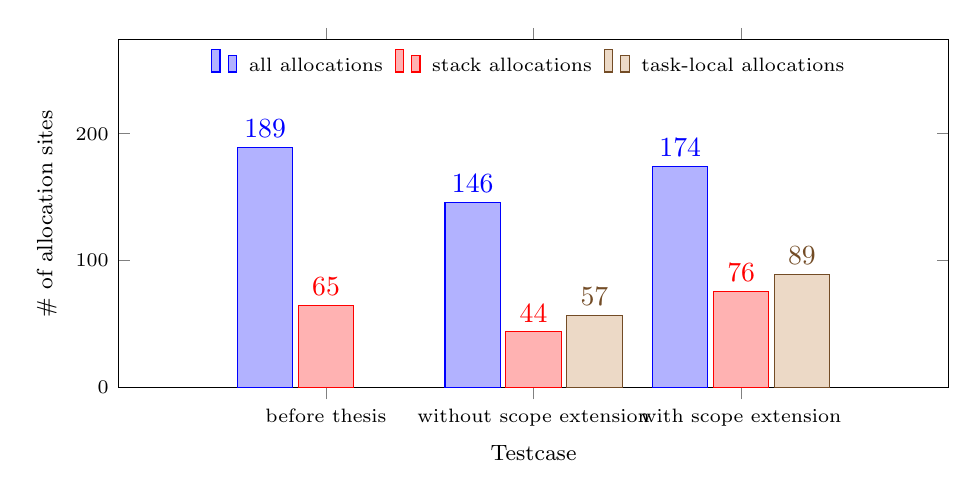
\begin{tikzpicture}%[auto, font=\footnotesize]
		\begin{axis}[
			width=\textwidth,
			height=6cm,
			ybar,
			bar width=20pt,
			ylabel=\# of allocation sites,
			xlabel=Testcase,
			enlarge x limits=0.5,
			ymin=0,
			enlarge y limits={value=0.45,upper},
			symbolic x coords={before thesis, without scope extension, with scope extension},
			xtick=data,
			nodes near coords,
			nodes near coords align={vertical},
			legend style={draw={none}, at={(0.5, 0.99)}, anchor={north}, legend columns=-1},
			legend cell align=left,
			label style={font=\footnotesize},
			tick label style={font=\scriptsize},
			legend style={font=\scriptsize}
		]
		  % all allocations
			\addplot coordinates {(before thesis, 189) (without scope extension, 146) (with scope extension, 174)};
			\addlegendentry{\;all allocations\;}
			\addplot coordinates {(before thesis, 65) (without scope extension, 44) (with scope extension, 76)};
			\addlegendentry{\;stack allocations\;}
			\addplot coordinates {(without scope extension, 57) (with scope extension, 89)};
			\addlegendentry{\;task-local allocations\;}
		\end{axis}
	\end{tikzpicture}
\end{document}
